\mysubsection{Message et communication asynchrone}

\ifbook{
  \mysubsubsection{Problématique de la communication asynchrone}
    \paragraph{} Depuis les débuts de l'informatique, le besoin d'une communication \textbf{asynchrone} entre
    deux processus ou deux programmes est présent et les problématiques liées à ce genre de communication sont
    bien connues. Il n'en reste pas moins que si tout langages de programmation donnent les primitives nécessaires
    à l'implémentation d'une telle communication, on fait plus souvent appel à des \textit{middlewares} dédié, le
    \textit{Message Oriented Middleware}, autant pour faciliter le développement qu'assurer une bonne gestion des
    messages.
}

\ifslide{
  \begin{frame}{Problématique de la communication asynchrone}
    \begin{block}{Motivations}
      \begin{itemize}
        \item \textit{fire and forget}
        \item \textit{can't wait}
        \item \textit{producteur / consommateur}
      \end{itemize}
    \end{block}
}

\ifbook{
 \paragraph{} Avant d'avancer plus en avant dans la description du fonctionnement générale de ces
 \textit{middlewares} étudions rapidement les cas d'utilisation qui motive leurs utilisations. Loin
 d'être exhaustive, voici une petit série d'exemple où l'on souhaite généralement mettre en place
 une communication \textbf{asynchrone} entre deux processus:
 \begin{itemize}
   \item [\textit{fire and forget}] Un processus souhaite communiquer une information à un autre,
   sans attendre que ce dernier est fini son traitement pour continuer (ex: journalisation des
   opérations d'une application). Généralement, dans ce genre de cas, le traitement qui doit être
   réalisé par le second processus n'a pas d'impact sur celui réalisé par le premier.
   \item [\textit{producteur et consommateur}] Problème d'algorithmique classique, le
   \mylink{http://fr.wikipedia.org/wiki/Mod\%C3\%A8le\_producteur-consommateur}{modèle
   producteur/consommateur} est un cas d'utilisation classique d'une communication asynchrone. En
   quelques mots, le processus producteur dépose, dès qu'il peut, une demande de traitement dans une
   sorte de "boite à message", qu'un processus consommateur, quand il le souhaitera ou pourra,
   récupérer.
 \end{itemize}
}


\ifslide{
    \begin{block}{Problématiques}
      \begin{itemize}
        \item gestion d'erreur
        \item gérer les queues
        \item persistance (ou non) des messages
      \end{itemize}
    \end{block}
  \end{frame}
}

\ifbook{

\paragraph{} La nature même de la communication induit rapidement le besoin de gérer l'état des
messages échangés. En effet, à partir du moment où la réception d'un message n'est pas immédiate,
il va souvent devenir nécessaire de s'assurer que ces derniers soit persistés et administrer. Ce
dernier point est un important, car si les messages ne sont jamais consommés par exemple, le
système peut rapidement se retrouver dans un état instable, car débordé de message qui ne
"disparaissent jamais"...

\paragraph{} Il devient rapidement nécessaire de gérer des files d'attentes (\textit{Queues} en
anglais) ainsi que des erreurs de transmission. Il apparait clairement que tout ceci offre là
encore, un terrain d'investigation intéressant pour la conception de \textit{middleware}...
}

\ifslide{

  \begin{frame}{Message Oriented Middleware (MOM)}
    \begin{block}{Domaines}
      \begin{itemize}
        \item Publish/Subscribe (pub/sub) : n producteurs, n consommateurs
        \item Point To Point (PTP) : n producteurs, 1 consommateur
      \end{itemize}
    \end{block}

    \begin{center}
      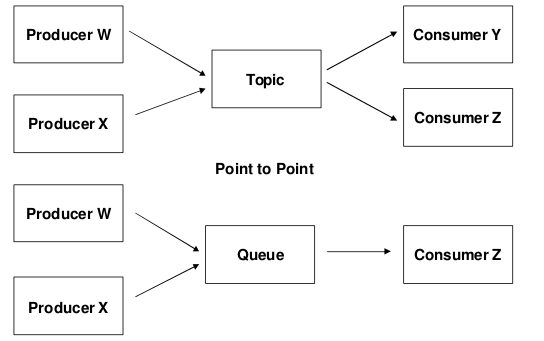
\includegraphics[scale=0.3]{img/topic-queue.png}
    \end{center}
  \end{frame}
}

\ifbook{

  \paragraph{} Un autre avantage des \textit{MOM} (\textit{Message Oriented Middleware}) est aussi la
  capacité d'effectuer une communication de 1 à n tiers aisément. En effet, une fois un message remis
  à tel programme, ce dernier peut aisément le mettre à disposition d'un comme de plusieurs
  processus. Ainsi, on peut aisément disposer de plusieurs processus (ou même machine) prête à
  consommer les messages transmis.

  \mysubsubsection{Un exemple de standardisation des MOM : Java Message Service}

 \paragraph{} Sans rentrer dans les détails de cette API Java\footnote{Voir
 \mylink{http://en.wikipedia.org/wiki/Java_Message_Service}{Java Message Service}}, nous
 pouvons juste retenir que, reprenant la théorie évoqué plus haut, cette spécification définit
 l'API que doit supporter et respecter un MOM.

 \paragraph{} En outre de fournir les services d'administration et de diffusion évoqués, cette
 API assure aussi un fort \textbf{découplage} entre le logiciel client (utilisant l'API) et
 l'implémentation de la spécification JMS qu'il utilise. Ceci permet ainsi de aisément remplacer
 une implémentation par une autre - sans altérer le comportement du programme\footnote{Bien
 évidemment selon les implémentations, les performances, comme les bogues présents varieront}.

 \paragraph{} Le schéma ci dessous présente, dans les grandes lignes, les composants logicielle
 impliqués lors d'une communication aynchrone utilisant JMS.

  \begin{center}
    \begin{figure}
      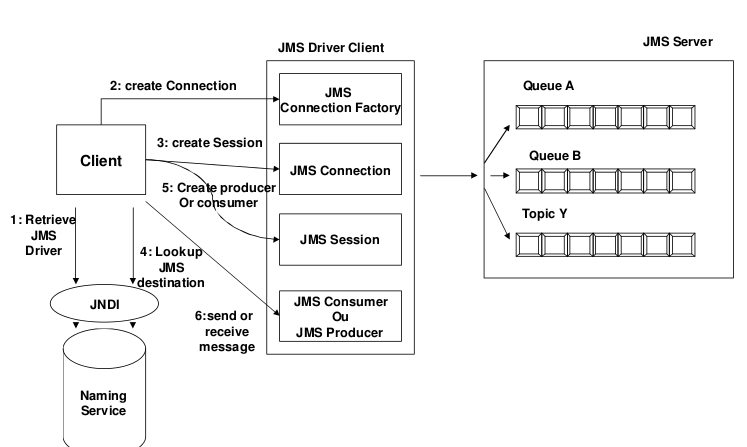
\includegraphics[scale=0.3]{img/jms-steps.png}
      \caption{Vue générale d'une communication asynchrone à l'aide de JMS}
    \end{figure}
  \end{center}
}

\ifslide{

   \begin{frame}
     \begin{block}{Invocation JMS}
       \begin{itemize}
         \item Localiser le driver JMS lookup JNDI. Le driver est une connection
 factory
         \item Créer une connection JMS obtenir une connection à partir de la
 connection factory
         \item Créer une session JMS :Il s'agit d'un objet qui va servir à recevoir et
 envoyer des messages. On l'obtient à partir de la connection.
         \item Localiser la destination JMS: Il s'agit du canal sur lequel les
 messages sont emis ou recus. Normalement, c'est réglé par le
 déployeur. On obtient la destination via JNDI.
         \item Créer un producteur ou un consommateur JMS. Utilisés pour écrire
 ou lire un message. On les obtient à partir de la destination et de la
 session.
         \item Envoyer ou recevoir un message
       \end{itemize}
     \end{block}
   \end{frame}

   \begin{frame}{Message Oriented Middleware (MOM)}
     \begin{center}
       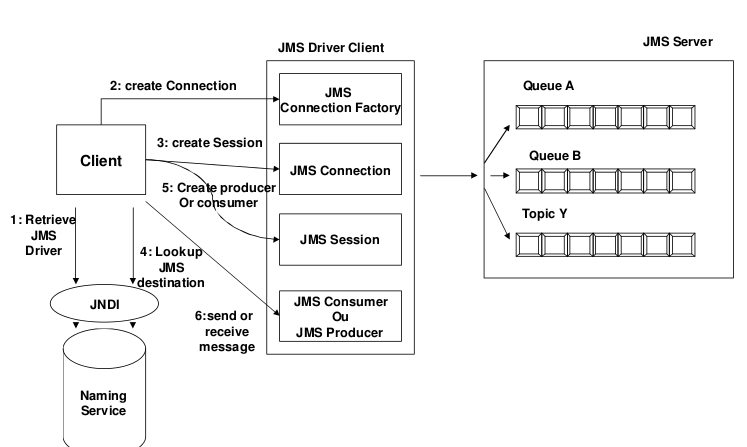
\includegraphics[scale=0.3]{img/jms-steps.png}
     \end{center}
   \end{frame}
 }

\ifslide{

  \begin{frame}{Message Oriented Middleware (MOM)}
    \begin{block}{Domaines}
      \begin{itemize}
        \item Transactions and MBD %: La production et la consommation du message sont dans deux transactions séparées...
        \item Sécurité %: Les MDB ne reçoivent pas les informations de sécurité du producteur avec le message.
      \end{itemize}
    \end{block}
  \end{frame}

  \begin{frame}
    \begin{block}{Advantages}
      \begin{itemize}
        \item message-based communications protocol
        \item store/buffer
        \item routing / load balancing
      \end{itemize}
    \end{block}
  \end{frame}

  \begin{frame}{Standardisation ?}
    \begin{block}{No Standard yet :( (API only) }
      \begin{itemize}
        \item JMS (Java Messaging System)
        \item MSMQ (Microsoft Message Queuing)
        \item Amazon Simple Queue Service
      \end{itemize}
    \end{block}

    \begin{block}{Protocol}
      \begin{itemize}
        \item AMQP (Advanced Message Queuing Protocol) - protocole
        \item STOMP (Streaming Text Oriented Messaging Protocol)
      \end{itemize}
    \end{block}
 \end{frame}
}

\demoframe{Communication Asynchrone}{Exemple avec JMS}
